%----------------------------------------------------------------------
%                   LATEX TEMPLATE FOR PhD THESIS
%----------------------------------------------------------------------
% based on Harish Bhanderi's PhD/MPhil template, then Uni Cambridge
% http://www-h.eng.cam.ac.uk/help/tpl/textprocessing/ThesisStyle/
% corrected and extended in 2007 by Jakob Suckale, then MPI-CBG PhD programme
% and made available through OpenWetWare.org - the free biology wiki
\documentclass[twoside,12pt]{Latex/Classes/PhDthesisPSnPDF}%,openany
\usepackage[final]{pdfpages}
\usepackage{amsmath}
\usepackage{amstext}
\usepackage{dsfont}
\usepackage{float}
\usepackage{caption}
\usepackage{subcaption}
\usepackage{rotating}
\usepackage{tabularx}
\usepackage{multirow}
\usepackage{booktabs}
\usepackage{lscape}
\usepackage{tikz}
\usepackage{rotating}
\usepackage{afterpage}
%\usepackage[table, xcdraw]{xcolor}
%\usepackage{mathptmx} %%%%%%%%%%%%%|%%%%%%%%%%%%%%%%%%%%%%%%%%%%%%%%%% comenten esta l?nea para volver a la letra original
%\spanishdecimal{.}
\usepackage[spanish]{babel}
%%%%%%%%%%%%%%%
\usepackage{listings}
\usepackage{color}
\lstset{language=Delphi,breaklines=true,basicstyle=\ttfamily,frame=single}%basicstyle=\tiny\ttfamily ... para c�digo peque�o
%\lstdefinestyle{customc}{
%  belowcaptionskip=1\baselineskip,
%  breaklines=true,
%  frame=L,
%  xleftmargin=\parindent,
%  language=C,
%  showstringspaces=false,
%  basicstyle=\footnotesize\ttfamily,
%  keyword style=\bfseries\color{green!40!black},
%  commentstyle=\itshape\color{purple!40!black},
%  identifierstyle=\color{blue},
%  stringstyle=\color{orange},
%}
%
%\lstdefinestyle{customasm}{
%  belowcaptionskip=1\baselineskip,
%  frame=L,
%  xleftmargin=\parindent,
%  language=[x86masm]Assembler,
%  basicstyle=\footnotesize\ttfamily,
%  commentstyle=\itshape\color{purple!40!black},
%}
%
%\lstset{escapechar=@,style=customc}
%%%%%%%%%%%
%\usepackage[latin1]{inputenc}
\hbadness=10000
\hfuzz=50pt
\let\olditemize\itemize
\def\itemize{\olditemize\itemsep=0pt }

%-----------------------Dedicatoria  n  , Resumen, Agradecimientos
\setlength\parindent{0pt}
\newcommand{\forceindent}{\leavevmode{\parindent=1em\indent}}
\usepackage{titlesec}
\spanishdecimal{.}
\usepackage[acronym,toc]{glossaries}
\makeglossaries

\begin{document}
\renewcommand\baselinestretch{1}
\baselineskip=15pt plus1pt
\pagenumbering{alph}
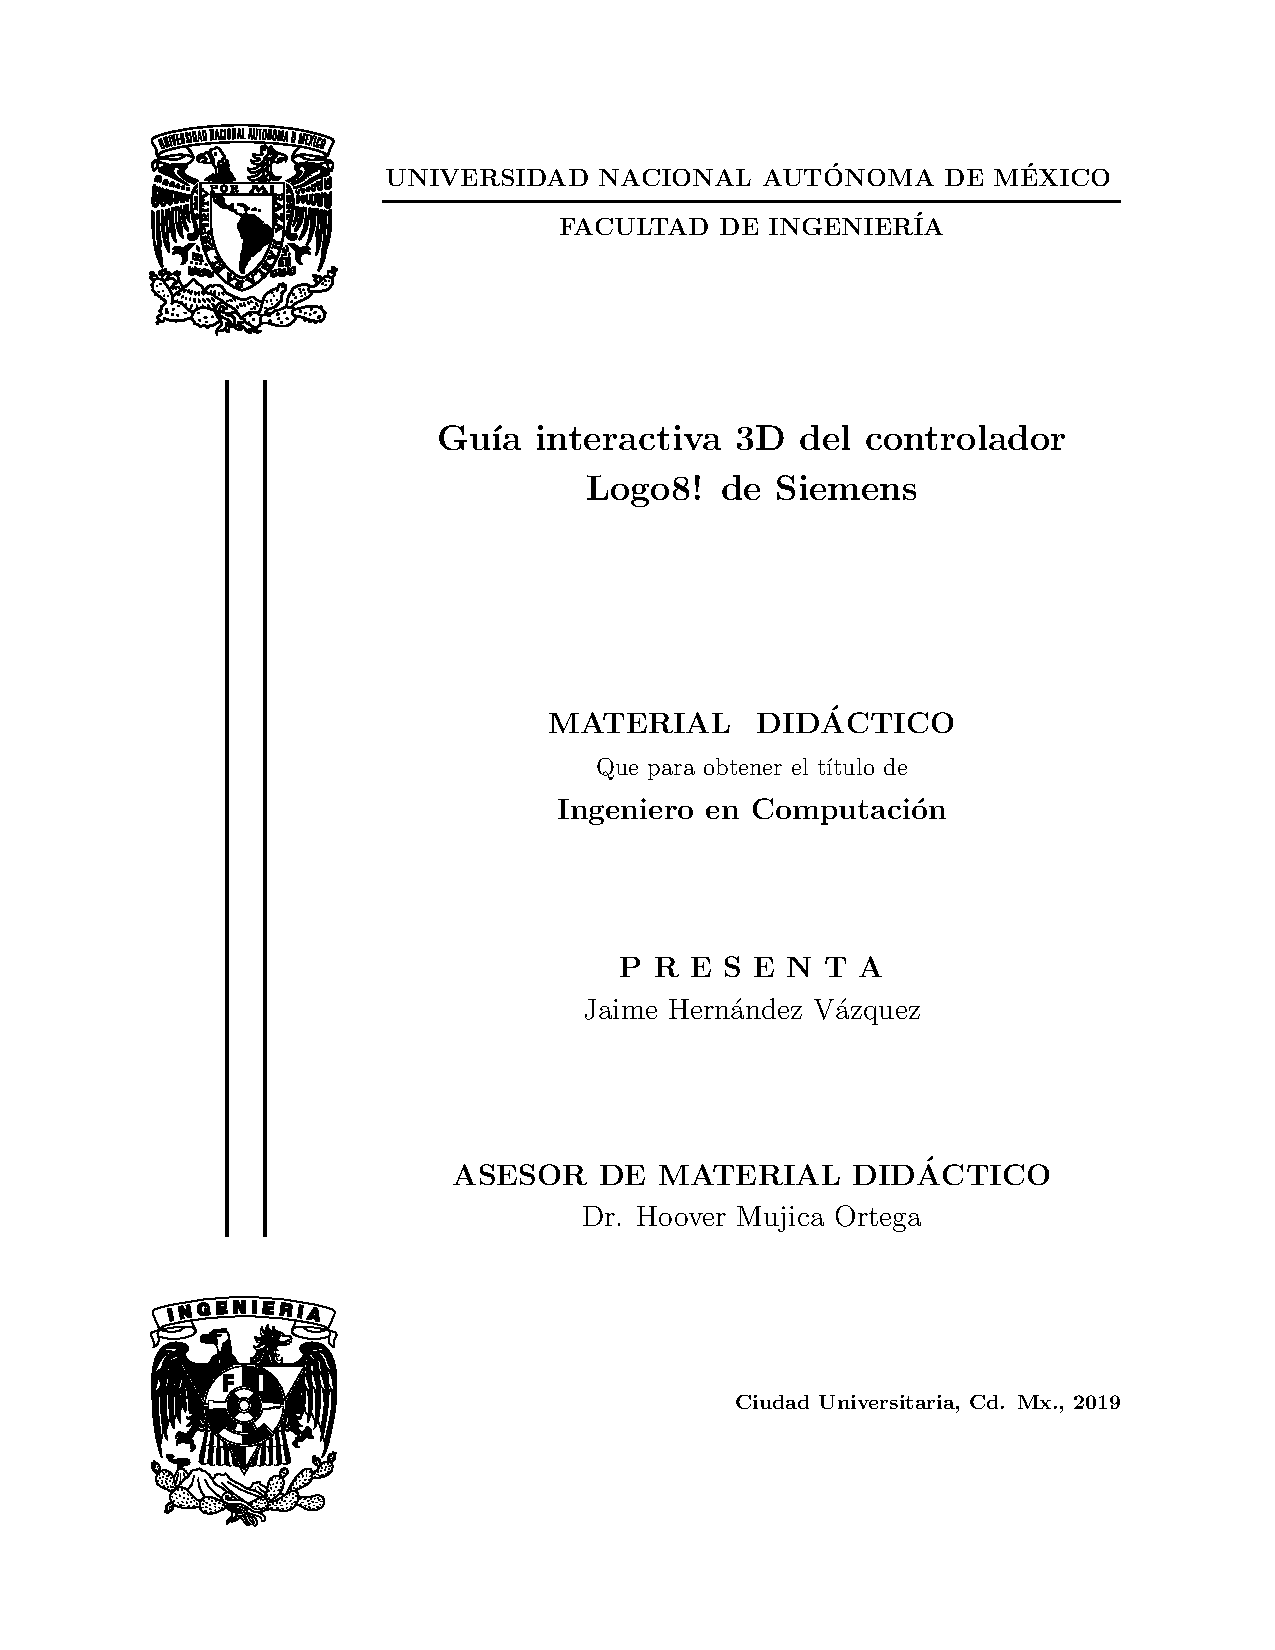
\includepdf[pages={1,2,3,4}]{0_portada/Portada_Final.pdf}
\frontmatter
%\include{1_Frontmatter/glossary}
\include{1_Frontmatter/acknowledgement}
\include{1_Frontmatter/dedication}
\include{1_Frontmatter/abstract}
%\include{1_Frontmatter/abstracteng}
\newtheorem{theorem}{{\bf Teorema}}[chapter]

%----------------------- Contenido
\renewcommand{\contentsname}{Contenido}
\setcounter{secnumdepth}{3} % organisational level that receives a numbers
\setcounter{tocdepth}{3}    % print table of contents for level 3
\tableofcontents            % print the table of contents
%----------------------- Lista de Figuras y Tablas
\listoffigures	% print list of figures
\cleardoublepage
\listoftables  % print list of tables
\cleardoublepage
%\printglossaries
%\cleardoublepage
%: --------------------- Glosario de T?rminos
\providecommand{\abs}[1]{\left\lvert#1\right\rvert}
\providecommand{\norm}[1]{\lVert#1\rVert}
\providecommand{\sign}[1]{sgn\left(#1\right)}
\include{1_Frontmatter/glossary}
\cleardoublepage
\printnomenclature
%--------------------------------------------------------------
%                  MAIN DOCUMENT SECTION
%--------------------------------------------------------------
\mainmatter
\renewcommand{\chaptername}{Cap�tulo} % uncomment to print only "1" not "Chapter 1"
\renewcommand{\bibname}{Referencias} %% changes the header; default: Bibliography
%: ----------------------- subdocuments ------------------------
\include{2_Cap_1_/Cap_1}
\include{3_Cap_2_/Cap_2}
\include{4_Cap_3_/Cap_3}
\include{5_Cap_4_/Cap_4}
\include{6_Cap_5_/Cap_5}
\include{7_Cap_6_/Cap_6}
\include{8_Apendice/Apendice}
% --------------------------------------------------------------
%:                  BACK MATTER: appendices, refs,..
% --------------------------------------------------------------
%\include{6_Apendice/Apendice}
% --------------------------------------------------------------
%: ----------------------- bibliography ------------------------
%\usepackage{setspace}
%\begin{spacing}{1.1}|
\renewcommand{\baselinestretch}{1.05}
\begin{small} % tiny(5) < scriptsize(7) < footnotesize(8) < small (9)
\bibliographystyle{Latex/Classes/apalike_Htec} % Title is link if provided
\bibliography{Bibliografia}
\end{small}
\end{document}

